%% ----------------------------------------------------------------
%% Thesis.tex -- MAIN FILE (the one that you compile with LaTeX)
%% ----------------------------------------------------------------



% Set up the document
\documentclass[a4paper, 11pt, oneside]{Style/UCLThesis}  % Use the "UCLThesis" style, based on the ECS Thesis style by Steve Gunn

%TC:macro \cmt [ignore]
%TC:macro \note [ignore]
\graphicspath{{Figures/}}  % Location of the graphics files (set up for graphics to be in PDF format)


% Include any extra LaTeX packages required
\usepackage[square, numbers, comma, sort&compress]{natbib}  % Use the "Natbib" style for the references in the Bibliography
\usepackage{verbatim}  % Needed for the "comment" environment to make LaTeX comments
\usepackage{Style/vector}  % Allows "\bvec{}" and "\buvec{}" for "blackboard" style bold vectors in maths
\hypersetup{urlcolor=blue, colorlinks=true}  % Colours hyperlinks in blue, but this can be distracting if there are many links.
\usepackage{booktabs}
\usepackage{tabularx}
\usepackage{ltablex}
\usepackage{setspace}
%\usepackage{fullpage}
\usepackage{listings}
\usepackage{amsmath}
\usepackage{color}
%\usepackage{dsfont}
\usepackage{multicol}
\usepackage{xcolor}
\usepackage{dirtree}
\usepackage{texshade}
\usepackage{subfigure}
\usepackage{graphicx,picture,calc}
\usepackage{wrapfig}
%\usepackage{lmodern} % Package appears to prevent {verbatim} and {listings} from displaying correctly
\usepackage{lscape}
\usepackage{tikz}
\usepackage{pifont}
\usepackage{fancyvrb}
%\usepackage{textcomp}
%\usepackage{array}

%\listfiles    % useful to check version of packages in the log

%% ----------------------------------------------------------------

\newcommand{\note}[1]{{\color{red} [*** Comment: #1 ***]}}

\begin{document}
\frontmatter	  % Begin Roman style (i, ii, iii, iv...) page numbering

% Set up the Title Page
\title  {Predicting and Characterising Zinc Metal Binding Sites in Proteins}
\authors  {\texorpdfstring
          {Sam M. Ireland}
          {Sam M. Ireland}
          }
\addresses  {\groupname\\\deptname\\\univname}  % Do not change this here, instead these must be set in the "Thesis.cls" file, please look through it instead
\date       {\today}
\subject    {}
\keywords   {}

\maketitle
%% ----------------------------------------------------------------

\setstretch{1.5}  % It is better to have smaller font and larger line spacing than the other way round

% Define the page headers using the FancyHdr package and set up for one-sided printing
\fancyhead{}  % Clears all page headers and footers
\rhead{\thepage}  % Sets the right side header to show the page number
\lhead{}  % Clears the left side page header

\pagestyle{fancy}  % Finally, use the "fancy" page style to implement the FancyHdr headers

%% ----------------------------------------------------------------
% Declaration Page required for the Thesis, your institution may give you a different text to place here
\Declaration{

\addtocontents{toc}{\vspace{1em}}  % Add a gap in the Contents, for aesthetics

I, SAM IRELAND, declare that this thesis titled, `Predicting and Characterising Zinc Metal Binding Sites in Proteins' and the work presented in it are my own. I confirm that:

\begin{itemize}
\item[\tiny{$\blacksquare$}] This work was done wholly or mainly while in candidature for a research degree at this University.

\item[\tiny{$\blacksquare$}] Where any part of this thesis has previously been submitted for a degree or any other qualification at this University or any other institution, this has been clearly stated.

\item[\tiny{$\blacksquare$}] Where I have consulted the published work of others, this is always clearly attributed.

\item[\tiny{$\blacksquare$}] Where I have quoted from the work of others, the source is always given. With the exception of such quotations, this thesis is entirely my own work.

\item[\tiny{$\blacksquare$}] I have acknowledged all main sources of help.

\item[\tiny{$\blacksquare$}] Where the thesis is based on work done by myself jointly with others, I have made clear exactly what was done by others and what I have contributed myself.
\\
\end{itemize}


Signed:\\
\rule[1em]{25em}{0.5pt}  % This prints a line for the signature

Date:\\
\rule[1em]{25em}{0.5pt}  % This prints a line to write the date
}
\clearpage  % Declaration ended, now start a new page

\begin{comment}
%% ----------------------------------------------------------------
% The "Funny Quote Page"
\pagestyle{empty}  % No headers or footers for the following pages

\null\vfill
% Now comes the "Funny Quote", written in italics
\textit{``A doughnut, my reign for a doughnut !!!''}

\begin{flushright}
*** AUTHOR NAME HERE ***
\end{flushright}

\vfill\vfill\vfill\vfill\vfill\vfill\null
\clearpage  % Funny Quote page ended, start a new page
\end{comment}
%% ----------------------------------------------------------------

% The Abstract Page
\chapter{Impact Statement}

This PhD has resulted in the creation of a dedicated database of zinc binding sites (ZincBindDB) and tools for easily accessing it, predictive models for predicting zinc binding sites in proteins (ZincBindPredict), and a novel Python library for analysing protein structures (atomium).

There was previously no such resource for collating zinc binding sites, and so the introduction of one facilitates research into zinc binding sites generally by giving researchers in this field a convenient, centralised repository of the sum of all knowledge of zinc binding sites for which there is structural information - where no such centralised repository existed before. This underpins and supports research into a diverse area of biology. The codebase is also open source and highly extensible, and could be expanded to support other metals as required.

Zinc binding is a property of about 10\% of proteins, and is particularly important in certain enzyme reactions. Knowing whether a protein binds to zinc can offer insights into its function, and knowing precisely where it binds zinc can show the mechanism by which it carries out its intended function, as well as provide suggestions as to how pharmaceutical molecules might disrupt or enhance this function where required for medical interventions. The tools developed here make it easier to computational assess whether a protein binds zinc, and where it does if so - aiding these endeavours.

The newly developed Python library atomium makes studying and analysing protein structures easier for Python programmers, specifically giving them the ability to study higher order assemblies of protein chains called biological assemblies, which was not possible with the existing BioPython library. This makes structural biology research more efficient.


\clearpage  % Abstract ended, start a new page
%% ----------------------------------------------------------------

% The Abstract Page
\addtotoc{Abstract}  % Add the "Abstract" page entry to the Contents
\abstract{
\addtocontents{toc}{\vspace{1em}}  % Add a gap in the Contents, for aesthetics

Zinc is one of the most important biologically active metals. Ten per cent of the human genome is thought to encode a zinc binding protein and its uses encompass catalysis, structural stability, gene expression and immunity. Knowing whether a protein binds to zinc can offer insights into its function, and knowing precisely where it binds zinc can show the mechanism by which it carries out its intended function, as well as provide suggestions as to how pharmaceutical molecules might disrupt or enhance this function where required for medical interventions. At present, there is no specific resource devoted to identifying and presenting all currently known zinc binding sites. This PhD has resulted in the creation of ZincBind --- a database of zinc binding sites (ZincBindDB), predictive models of zinc binding at the family level (ZincBindPredict) and a user-friendly, modern website frontend (ZincBindWeb). Both ZincBindDB and ZincBindPredict are also available as GraphQL APIs. The database of zinc binding sites currently contains 38,141 sites, and is automatically updated every week. The predictive models, trained using the Random Forest Machine Learning algorithm, all achieve an MCC $\ge$ 0.88, recall $\ge$0.93 and precision $\ge$0.91 for the structural models (mean MCC = 0.97), while the sequence models have MCC $\ge$ 0.64, recall $\ge$0.80 and precision $\ge$0.83 (mean MCC = 0.87), outperforming competing, previous predictive models.
}

\clearpage  % Abstract ended, start a new page
%% ----------------------------------------------------------------

\setstretch{1.3}  % Reset the line-spacing to 1.3 for body text (if it has changed)

% The Acknowledgements page, for thanking everyone
\acknowledgements{
\addtocontents{toc}{\vspace{1em}}  % Add a gap in the Contents, for aesthetics

I am enormously grateful to the Wellcome Trust who, in addition to funding the entirety of this PhD and its associated costs, provided considerable assistance and understanding during the COVID pandemic with their prompt, targeted response.

I am greatly indebted to my supervisor, Professor Andrew Martin. Enormously helpful with questions, feedback and guidance at every stage of this project, while still granting me almost complete oversight of the direction and management of the project itself --- I could not have asked for a friendlier, reliable and domain-knowledgable primary supervisor.

Likewise I am grateful to my second supervisor, Professor Stephen Perkins, and my thesis chair, Professor Christine Orengo, whose feedback and contributions at our many meetings were helpful to the eventual success of the project.

Prior to the start of the project I completed three rotations as part of this programme, and the help, guidance, and above all welcoming nature of those three supervisors --- Professor Stephen Perkins (again), Professor Bonnie Wallace, and Professor Francesco Gervasio, to whom I partly owe the relative ease with which I was able to settle into PhD life --- should be noted.

Indeed I would particularly like to single out the Postdoc Dr. Altin Sula, of Professor Bonnie Wallace's lab, whose patience, knowledge, mentorship and generosity of time was invaluable in making that second rotation the considerable success that it was --- particularly given my relative lack of wet lab experience going into it.

More generally I am grateful to my fellow PhD Students and other colleagues at UCL and the Institute of Structural and Molecular Biology for their help, insights and comradeship.

Finally, I am indebted to the countless researchers and technicians who, over the past five decades, have painstakingly populated the Protein Data Bank with structures. Each of the tens of thousands of structures which a computational biologist such as myself considers for a fraction of a second was the work of months of highly skilled labour by teams of people who I will never meet or know, but by whose endeavours this project and the many like it are made possible. Thanks.

}
\clearpage  % End of the Acknowledgements
%% ----------------------------------------------------------------

\pagestyle{fancy}  %The page style headers have been "empty" all this time, now use the "fancy" headers as defined before to bring them back

%% ----------------------------------------------------------------
\lhead{\emph{Contents}}  % Set the left side page header to "Contents"
\tableofcontents  % Write out the Table of Contents

%% ----------------------------------------------------------------
\lhead{\emph{List of Figures}}  % Set the left side page header to "List of Figures"
\listoffigures  % Write out the List of Figures

%% ----------------------------------------------------------------
\lhead{\emph{List of Tables}}  % Set the left side page header to "List of Tables"
\listoftables  % Write out the List of Tables

%% ----------------------------------------------------------------

%% ----------------------------------------------------------------
\begin{comment}
\clearpage  %Start a new page
\lhead{\emph{Symbols}}  % Set the left side page header to "Symbols"
\listofnomenclature{lll}  % Include a list of Symbols (a three column table)
{
% symbol & name & unit \\
$a$ & distance & m \\
$P$ & power & W (Js$^{-1}$) \\
& & \\ % Gap to separate the Roman symbols from the Greek
$\omega$ & angular frequency & rads$^{-1}$ \\
}

%% ----------------------------------------------------------------
% End of the pre-able, contents and lists of things
% Begin the Dedication page

\setstretch{1.5}  % Return the line spacing back to 1.5

\pagestyle{empty}  % Page style needs to be empty for this page
\dedicatory{For/Dedicated to/To my\ldots}

\addtocontents{toc}{\vspace{2em}}  % Add a gap in the Contents, for aesthetics

\end{comment}

%% ----------------------------------------------------------------
\mainmatter	  % Begin normal, numeric (1,2,3...) page numbering
\pagestyle{fancy}  % Return the page headers back to the "fancy" style

% \includeonly{.....}


%%%% MACRO DEFINITION %%%%

\providecommand{\pvivax}{P.~vivax}
\providecommand{\pfalciparum}{P.~falciparum}
\providecommand{\cterm}{C-terminus}
\providecommand{\nterm}{N-terminus}

\providecommand{\e}[1]{\ensuremath{\times 10^{#1}}}
\newcolumntype{P}[1]{>{\centering\arraybackslash}p{#1}}
\newcolumntype{M}[1]{>{\centering\arraybackslash}m{#1}}

\providecommand{\refimage}[1]{\figurename~\ref{fig:#1}}

% figure that is as wide as the text
\newcommand{\insertfigure}[5][1]{
\begin{figure}[h!]
	\makebox[\textwidth]{\includegraphics[width=#1\textwidth]{Chapter1_pics/#2}}
	\caption[#3]{\small{#4}}\label{fig:#5}
\end{figure}
}

%TC:macro \note [ignore]



%%%%%%%%%%%%%%%%%%%%%%%%%%%%%%%%%%%%%%%%%%%%%%%%%%%%%%%%%%%%%%%%%%%%%%%%%%%%%%%%%%%%%%%%%%%%%%%%%%%%%%%%%%%%%%%%%%%%%
%%%%%%%%%%%%%%%%%%%%%%%%%%%%%%%%%%%%%%%%%%%%%%%%%%%%%%%%%%%%%%%%%%%%%%%%%%%%%%%%%%%%%%%%%%%%%%%%%%%%%%%%%%%%%%%%%%%%%
%													BEGIN
%%%%%%%%%%%%%%%%%%%%%%%%%%%%%%%%%%%%%%%%%%%%%%%%%%%%%%%%%%%%%%%%%%%%%%%%%%%%%%%%%%%%%%%%%%%%%%%%%%%%%%%%%%%%%%%%%%%%%
%%%%%%%%%%%%%%%%%%%%%%%%%%%%%%%%%%%%%%%%%%%%%%%%%%%%%%%%%%%%%%%%%%%%%%%%%%%%%%%%%%%%%%%%%%%%%%%%%%%%%%%%%%%%%%%%%%%%%

\chapter{Introduction} % Write in your own chapter title
\label{Chapter1}
\lhead{Chapter 1. \emph{Introduction}} % Write in your own chapter title to set the page header

Proteins are polymer chains of amino acid residues, and while the chemical diversity of the twenty canonical amino acids utilised in Biology can offer proteins a staggering variety of folds and functionality, there remain chemical processes that are not possible using only this chemical species. Consequently, many proteins use cofactors. These are chemicals which associate with the protein but are not generally covalently bound to them.

In order for a protein to induce this association to happen, it must present a region of its surface that the cofactor in question will experience an attraction to, and for which association will be thermodynamically favourable. The residues that make up this attractive region are called binding sites.

Metal atoms are a common cofactor. In this case the binding site is a metal binding site, and when the metal is zinc we can speak of a `zinc binding site'.

Clearly, zinc will only experience an attraction towards certain kinds of protein surfaces, and so proteins which need to attract a zinc cofactor will have to present surface residues capable of doing this. It should be possible to predict, therefore, whether a protein's structure has a potential zinc binding site on it. Furthermore, because structure is determined by amino acid sequence, it should in principle be possible to predict zinc binding capabilities from protein sequence.

This PhD project is an attempt to develop novel methods for doing so.

\section{Zinc}

Any investigation into the phenomenon of zinc binding to proteins must begin with a look at zinc and its properties.

\subsection{Transition Metals}

Transition metals are often employed as cofactors by proteins, particularly in catalysis. They occupy a different region of electron configuration space than the organic, non-metal atoms that make up the biological amino acids, and so can provide functionality that would otherwise be unavailable.

For example, by definition they have partially filled d-orbitals, which means that they can adopt a number of stable electron numbers each associated with a different charge, known as the different oxidation states. They can all lose their two 4s electrons to become 2+ in charge, but they can usually lose some of their d-electrons too. Iron for example has six d-electrons in its neutral state, and as five d-electrons each in its own orbital is relatively stable, it can also lose one of these d-electrons too, meaning that it can have a charge of 3+ or 2+. These different redox states are very useful when it comes to catalysis, because they can act as temporary custodians of electrons while the reaction substrates are in their intermediate states.

As cations, the transition metals also act as efficient Lewis acids - they can accept lone pairs of electrons. This is also useful in catalysis as it can stabilise intermediate structures by withdrawing excessive negative charge from them.

\note{Also explain how ligand/crystal stabilisation energy works, and breaking of degeneracy}

Unsurprisingly then, many proteins have evolved to take advantage of these useful properties of transition metals by presenting binding sites on their surface that will acquire one of them. This is generally done by bringing residues with available lone pairs into close proximity to each other, in an arrangement that matches the dimensions and orbital geometry of the desired metal.

\subsection{Zinc's Unique Properties}

Though a transition metal in the sense that it ten d-electrons but no 4p electrons, it is an unusual one - to the point where it is often not even classified as one. Many of the properties of transition metals derive from \emph{partially filled} d-orbitals, which zinc does not have. The five fully filled d-orbitals are relatively stable, meaning it can only really be oxidised to 2+ by losing its 4s electrons, so it has just one oxidation state. Electrons cannot be `promoted' from one d-orbital to another in solution as all spaces in the orbitals are already filled, so it has no colour or spectroscopic activity when in solution. At first glance, zinc would appear to be rather unremarkable metal, unworthy of much consideration by evolution.

However, the data show otherwise. About 10\% of all proteins in the human genome are zinc proteins with a zinc binding site - the second most abundant such metal after iron. It is also the only metal found in all classes of enzyme. Clearly, evolution has found zinc very useful.

In fact it is precisely that unremarkableness that has made zinc so attractive. Having just one oxidation state may mean that it cannot hold onto an electron mid-reaction, but it also means that the ion will retain its electronic properties in a wide range of reducing environments - and its status as a particularly good Lewis acid means it is still very useful in catalysis. Its lack of spectroscopic activity may make zinc solutions colourless, but the same arrangement of d-orbitals that causes this also means that there is no energetic penalty for zinc coming out of solution (where it is octahedrally coordinated) and into the binding site \note{Explain this MUCH better}.

\section{Predicting Zinc Binding}

There are still many proteins whose function is unknown. In many cases we only know their sequence, though some of these have had their structure solved experimentally.

One means of determining what function a protein might be intended to perform is to look for certain motifs associated with a given function. If, for example, it can be shown that such a protein had one or more zinc binding sites, that could offer insights into what function the protein performs. Indeed, that is ultimately the goal of this project.

Owing to this clear usefulness, there have been a number of attempts to develop such predictors in the past, dating back to the early 1990s. These methods and techniques form the essential context in which my own project should be understood, and also provide the benchmark of success against which my methods should be judged. Here their progress will be reviewed. They can essentially be divided into two broad categories - prediction from structure and prediction from sequence.

\subsection{Prediction from Structure}

Predicting zinc binding from structure takes the atom coordinates of some protein as its input, and produces as output residues in that structure which are believed to be able to bind zinc if zinc were present - generally along with some estimated probability that this should be the case.

This is perhaps of only limited utility, as very often proteins which can bind zinc tightly will have zinc bound when the structure is solved, and so no prediction is required. Where such methods are of use however is when a protein capable of binding zinc is crystallised without zinc being present - presumably because the researchers didn't know it could bind zinc and so did not provide any in the medium. These apoproteins can be scanned by predictors like this to identify unfilled zinc binding sites. \note{NMR invisibility?}

\note{Other uses?}

The earliest attempt at a general purpose prediction algorithm was the Hydrophobic Contrast Function, developed in 1990 \cite{yamashita1990metal} to detect metal binding sites in general. This began from the observation that metal atoms tended to be surrounded by a shell of hydrophilic atoms, which in turn were surrounded by an outer shell of hydrophobic atoms. They developed a function which took as its input a coordinate in space, and returned a measure of this `hydrophobic contrast' at that location. They showed that by scanning every point in the structure on a grid, evaluating the function at every point, and then ranking the points by their score (the function returned values between -1 for inverted contrast and 1 for desired contrast), the highest scoring points would be clustered at sites of metal binding.

This was the first demonstration that a property of metal binding sites could be used to create a predictive model. However it should be noted that it was only tested on structures with metals already present, not on apoproteins, and the initial observation itself was based on a very small number of metal proteins that were available at that time. It was later expanded upon by combining it with a template-based searching algorithm, whereby the known metal binding sites were represented as stripped-down `templates' of just alpha and beta carbons, and used to search proteins using a simple pattern matching algorithm \cite{gregory1993prediction}. Once a set of three residues matching a known template was found, the hydrophobic contrast function was applied to verify that the binding site was a region of high contrast, which it generally was. This was part of a pipeline for engineering binding sites into proteins, so it didn't require the matching residues to be of any particular type, but the general principle of using known site geometry and hydrophobic contrast properties to look in new structures was still in use.

\emph{MetSite}

\emph{Fold-X}

\emph{Goyal and Mande}

\emph{CHED}

\emph{FEATRUE}

\emph{SitePredict}

One of the more recent algorithms for identifying potential zinc binding sites in protein structures is TEMSP \cite{zhao2011structure}. This is actually reminiscent of some of the earlier work on this problem, in that it uses simple geometric patterns of known zinc binding sites - specifically their alpha and beta carbons - to search target structures without any particular machine learning method employed (though there is a certain amount of parameter training). Here the problem is simplified by creating a library of `residue pairs', where for each zinc binding site obtained from the PDB, they store each pairwise combination of liganding residues (actually just certain properties of them, such as alpha-alpha distance etc.) and then search the target protein for these. Once one is found, other template pairs are superimposed on the structure to find additional liganding residues. They used a stricter definition of `true positive' than previous attempts, and still reported a sensitivity of 86.0\% and a selectivity of 95.9\% in their test dataset - barely lower than the values obtained when testing on the training dataset used to refine their parameters. When applying their tool to a dataset of proteins of unknown function, they found some very promising results - finding 186 probable zinc binding sites. \note{So what?} Unfortunately, the online version of this tool is no longer accessible at time of writing.

\subsection{Prediction from Sequence}

%\insertfigure[0.5]{name.eps}{short caption}{long caption}{label}
% N.B. do not \end{document} at the end of the chapters

%%%% MACRO DEFINITION %%%%

\providecommand{\pvivax}{P.~vivax}
\providecommand{\pfalciparum}{P.~falciparum}
\providecommand{\cterm}{C-terminus}
\providecommand{\nterm}{N-terminus}

\providecommand{\e}[1]{\ensuremath{\times 10^{#1}}}
\newcolumntype{P}[1]{>{\centering\arraybackslash}p{#1}}
\newcolumntype{M}[1]{>{\centering\arraybackslash}m{#1}}

\providecommand{\refimage}[1]{\figurename~\ref{fig:#1}}

%TC:macro \note [ignore]



%%%%%%%%%%%%%%%%%%%%%%%%%%%%%%%%%%%%%%%%%%%%%%%%%%%%%%%%%%%%%%%%%%%%%%%%%%%%%%%%%%%%%%%%%%%%%%%%%%%%%%%%%%%%%%%%%%%%%
%%%%%%%%%%%%%%%%%%%%%%%%%%%%%%%%%%%%%%%%%%%%%%%%%%%%%%%%%%%%%%%%%%%%%%%%%%%%%%%%%%%%%%%%%%%%%%%%%%%%%%%%%%%%%%%%%%%%%
%													BEGIN
%%%%%%%%%%%%%%%%%%%%%%%%%%%%%%%%%%%%%%%%%%%%%%%%%%%%%%%%%%%%%%%%%%%%%%%%%%%%%%%%%%%%%%%%%%%%%%%%%%%%%%%%%%%%%%%%%%%%%
%%%%%%%%%%%%%%%%%%%%%%%%%%%%%%%%%%%%%%%%%%%%%%%%%%%%%%%%%%%%%%%%%%%%%%%%%%%%%%%%%%%%%%%%%%%%%%%%%%%%%%%%%%%%%%%%%%%%%

\chapter{Computational Techniques} % Write in your own chapter title
\label{Chapter2}
\lhead{Chapter 2. \emph{Computational Techniques}} % Write in your own chapter title to set the page header
In this chapter, the pre-existing algorithms and other computational techniques used to predict Zinc Binding Sites will be outlined.

It will not provide details of specific implementations of them used in this project, or any novel tecnhniques developed - those will be presented in later chapters. It is instead meant to give a general mathematical background to these techniques, and familiarise the reader with the terms that will be used in later chapters.
%%%% MACRO DEFINITION %%%%

\providecommand{\pvivax}{P.~vivax}
\providecommand{\pfalciparum}{P.~falciparum}
\providecommand{\cterm}{C-terminus}
\providecommand{\nterm}{N-terminus}

\providecommand{\e}[1]{\ensuremath{\times 10^{#1}}}
\newcolumntype{P}[1]{>{\centering\arraybackslash}p{#1}}
\newcolumntype{M}[1]{>{\centering\arraybackslash}m{#1}}

\providecommand{\refimage}[1]{\figurename~\ref{fig:#1}}

%TC:macro \note [ignore]



%%%%%%%%%%%%%%%%%%%%%%%%%%%%%%%%%%%%%%%%%%%%%%%%%%%%%%%%%%%%%%%%%%%%%%%%%%%%%%%%%%%%%%%%%%%%%%%%%%%%%%%%%%%%%%%%%%%%%
%%%%%%%%%%%%%%%%%%%%%%%%%%%%%%%%%%%%%%%%%%%%%%%%%%%%%%%%%%%%%%%%%%%%%%%%%%%%%%%%%%%%%%%%%%%%%%%%%%%%%%%%%%%%%%%%%%%%%
%													BEGIN
%%%%%%%%%%%%%%%%%%%%%%%%%%%%%%%%%%%%%%%%%%%%%%%%%%%%%%%%%%%%%%%%%%%%%%%%%%%%%%%%%%%%%%%%%%%%%%%%%%%%%%%%%%%%%%%%%%%%%
%%%%%%%%%%%%%%%%%%%%%%%%%%%%%%%%%%%%%%%%%%%%%%%%%%%%%%%%%%%%%%%%%%%%%%%%%%%%%%%%%%%%%%%%%%%%%%%%%%%%%%%%%%%%%%%%%%%%%

\chapter{ZincBind - The Database of Zinc Binding Sites} % Write in your own chapter title
\label{Chapter2}
\lhead{Chapter 2. \emph{ZincBind - The Database of Zinc Binding Sites}} % Write in your own chapter title to set the page header

This project is an attempt to develop novel means of predicting Zinc Binding Sites using the known properties of previously identified Zinc Binding Sites. As such, the initial step was to create a dataset of these already known sites.

This is an undertaking that has been performed previously - several times (see Chapter 1). One of the primary reasons that the effort has been duplicated so many times is because in none of the previous dataset generations did the authors make their data publicly available in an easy-to-use resource. Therefore from the very beginning of this project, the intention was always to not \emph{just} create this dataset of Zinc Binding Sites, but to make this database publicly available via a web resource, that would be continually updated with new sites as they become available.

This chapter will describe the creation of that dataset, and the web application that offers users access to the data - ZincBind.
%%%% MACRO DEFINITION %%%%

\providecommand{\pvivax}{P.~vivax}
\providecommand{\pfalciparum}{P.~falciparum}
\providecommand{\cterm}{C-terminus}
\providecommand{\nterm}{N-terminus}

\providecommand{\e}[1]{\ensuremath{\times 10^{#1}}}
\newcolumntype{P}[1]{>{\centering\arraybackslash}p{#1}}
\newcolumntype{M}[1]{>{\centering\arraybackslash}m{#1}}

\providecommand{\refimage}[1]{\figurename~\ref{fig:#1}}

%TC:macro \note [ignore]



%%%%%%%%%%%%%%%%%%%%%%%%%%%%%%%%%%%%%%%%%%%%%%%%%%%%%%%%%%%%%%%%%%%%%%%%%%%%%%%%%%%%%%%%%%%%%%%%%%%%%%%%%%%%%%%%%%%%%
%%%%%%%%%%%%%%%%%%%%%%%%%%%%%%%%%%%%%%%%%%%%%%%%%%%%%%%%%%%%%%%%%%%%%%%%%%%%%%%%%%%%%%%%%%%%%%%%%%%%%%%%%%%%%%%%%%%%%
%													BEGIN
%%%%%%%%%%%%%%%%%%%%%%%%%%%%%%%%%%%%%%%%%%%%%%%%%%%%%%%%%%%%%%%%%%%%%%%%%%%%%%%%%%%%%%%%%%%%%%%%%%%%%%%%%%%%%%%%%%%%%
%%%%%%%%%%%%%%%%%%%%%%%%%%%%%%%%%%%%%%%%%%%%%%%%%%%%%%%%%%%%%%%%%%%%%%%%%%%%%%%%%%%%%%%%%%%%%%%%%%%%%%%%%%%%%%%%%%%%%

\chapter{Predicting Zinc Binding Sites in Structures} % Write in your own chapter title
\label{Chapter4}
\lhead{Chapter 4. \emph{Predicting Zinc Binding Sites in Structures}} % Write in your own chapter title to set the page header

The aim of this component of the PhD is to create a system which ultimately is quite simple --- it would take as its input a protein structure, and output a list of zero or more residue combinations which are predicted to form a zinc binding site, with an accompanying probability.

This system is a machine learning system - it uses binary classifiers trained on the large dataset of zinc binding sites described in the previous chapter which `learn' what zinc binding sites look like form that data.

This chapter will describe the approach taken to solving this problem, the models created, the archietcture of the system from the user's point of view, and how the models are accessed and used.

\section{Families}

The first consideration when creating a machine learning classifier is the features that will be used to represent the inputs. Classifiers take their inputs as a vector of numbers and then try to assign the vector to one of two (in the case of binary classifiers) categories. Because the aim here is not just to label an entire protein as either zinc binfing or not zinc binding, but rather to identify the actual zinc binding residues, the proteins themselves are not the inputs - potential zinc binding sites within the protein are.

The main approach is to use combinations of residues as the inputs. That is all plausible combinations of residues will be looked at in turn, turned into a vector, and passed to the model.

Rather than create a single model, the decision was taken early on to create a model for each family. That is, there is a model which looks at sets of three histidines and tries to determine if it is a H3 binding site, a model which looks at sets of four cysteines and tries to determine if it is a C4 binding site, and so on. The main reason for this is that the geometric spacing of residues varies widely between different families, but not within families, which should allow a model to more easily learn what constitutes a likely binding site of a particular family. \note{Definitely need to show this in chapter 3!}

Another advnatage of this approach is a purely practical one. All the possible H3 binding sites in a protein are found by taking all combinations of three histidine residues, and while the combinatorics of this can lead to large numbers of potential sites to check, it is vastly smaller than the combinations of \emph{all} residues that would need to be checked if the model was suppoed to look for a generic zinc binding sites --- an infeasible task for all but the smallest of proteins.

\section{Datasets}
A training dataset was created for each family, using the ZincBindDB API. For each family, all zinc binding sites of that family, belonging to PDBs with a resolution equal to or better than 2 {\AA} were identified --- this quality cutoff being used so that the interatomic distances used in the making of the dataset could be relied upon.

For each site, the PDB file was downloaded.


\section{Old}


Before applying machine learning methods to the dataset, it is worth stopping to see if there are any straightforward identifiable geometric patterns that occur in the zinc binding stuctures gathered, which might be used as templates to search in unknown structures.

There is a wide variety of different binding modes and residue composition, as has been shown, so it is not at first apparent that there should be any usable geometric templates that can be extracted from these. However ZincBind divides the binding sites among families, each with their own residue makeup, and it seems much more plausible that there may be consistent within families. That is, while there may not be a single `zinc binding pattern', there may be a `H3' pattern for example, or a `C2H2' pattern.

Specifically, in this chapter I am interested in patterns of alpha and beta carbons, and the binding sites will be examined in terms of the geometry of these atoms. There are two primary reasons for this:

\begin{enumerate}
   \item The primary use case for searching through protein structures looking for zinc binding patterns is for when the structure is an apo-structure - without zinc. The actual liganding `tips' of liganding residues would be expected to vary more markedly in position than the alpha and beta carbons, which are more constrained by the overall fold of the protein \note{Cite!}.
   \item All residues contain alpha carbons, and all but one contain beta carbons. This means that essentially all residues can be searched for the resultant pattern. While this is not especially useful for the specific use case of finding native zinc binding sites, it \emph{is} useful for zinc binding site engineering. The pattern search could identify all residues which fit a given pattern, and if the residue identities also match it can be flagged as a possible zinc binding site, and if they don't, it can be flagged as a site which could feasibly be mutated to become one.
\end{enumerate}

\subsection{Profile Generation}

The initial step is to go through the ZincBind dataset and create a `profile' for each family. As some of the smaller families are quite esoteric, with large numbers of residues and metals, I decided to limit the scan for the smaller, more highly represented families. Specifically, the initial families were H3 (chosen because carbonic anhydrase is in this family, which is a frequent target of protein engineering), C4 (the most common family), C2H2, and C3H1 (both common families, important in zinc fingers).

Limiting to families which generally ligate a single zinc, rather than coactive binding sites, is important as there would be more constraints on residue position if they are all clustered around a single centre.

For each family, all sites are examined providing (1) their resolution is better than 2.5 ~{\AA}, (2) they only have a single metal, and (3) they ligate using side chain atoms \note{Not at time of writing!}.

The key attributes to determine for any given site are thos eattributes which would be used to actually search a novel structure. This means that the distribution of distances between residue atoms and the metal atom, however interesting, are irrelevant for these purposes because the structures being searched will not have metals present. That leaves the distances between the alpha and beta carbons themselves.

The number of measurements needed for a given binding site will increase with the number of residues, because all combinations need to be considered. For three residue sites such as H3, there are three measurements for the alpha carbons (CA1-CA2, CA2-CA3, CA1-CA3) and three for the beta carbons (CB1-CB2, CB2-CB3, CB1-CB3), for a total of six measurements. For four residue sites, there are six alpha measurements and six beta measurements \note{Give combinations formula explanation}.

This requires a certain consistency in which residues are labelled as 1, 2 etc. In this system, the residues of a given type are ordered by alpha carbon distance to the metal, and numbered accordingly.
%%%% MACRO DEFINITION %%%%

\providecommand{\pvivax}{P.~vivax}
\providecommand{\pfalciparum}{P.~falciparum}
\providecommand{\cterm}{C-terminus}
\providecommand{\nterm}{N-terminus}

\providecommand{\e}[1]{\ensuremath{\times 10^{#1}}}
\newcolumntype{P}[1]{>{\centering\arraybackslash}p{#1}}
\newcolumntype{M}[1]{>{\centering\arraybackslash}m{#1}}

\providecommand{\refimage}[1]{\figurename~\ref{fig:#1}}

%TC:macro \note [ignore]



%%%%%%%%%%%%%%%%%%%%%%%%%%%%%%%%%%%%%%%%%%%%%%%%%%%%%%%%%%%%%%%%%%%%%%%%%%%%%%%%%%%%%%%%%%%%%%%%%%%%%%%%%%%%%%%%%%%%%
%%%%%%%%%%%%%%%%%%%%%%%%%%%%%%%%%%%%%%%%%%%%%%%%%%%%%%%%%%%%%%%%%%%%%%%%%%%%%%%%%%%%%%%%%%%%%%%%%%%%%%%%%%%%%%%%%%%%%
%													BEGIN
%%%%%%%%%%%%%%%%%%%%%%%%%%%%%%%%%%%%%%%%%%%%%%%%%%%%%%%%%%%%%%%%%%%%%%%%%%%%%%%%%%%%%%%%%%%%%%%%%%%%%%%%%%%%%%%%%%%%%
%%%%%%%%%%%%%%%%%%%%%%%%%%%%%%%%%%%%%%%%%%%%%%%%%%%%%%%%%%%%%%%%%%%%%%%%%%%%%%%%%%%%%%%%%%%%%%%%%%%%%%%%%%%%%%%%%%%%%

\chapter{Predicting Zinc Binding Sites} % Write in your own chapter title
\label{Chapter5}
\lhead{Chapter 5. \emph{Predicting Zinc Binding in Proteins}} % Write in your own chapter title to set the page header

The aim of this part of the PhD is to create a system which conceptually is quite simple --- it would take as its input a protein sequence or protein sequence, and output a list of zero or more residue combinations which are predicted to form a zinc binding site, with an accompanying probability.

This system is a machine learning system - it uses binary classifiers trained on the large dataset of zinc binding sites described in the previous chapter which `learn' what zinc binding sites look like from that data.

This chapter will describe the approach taken to solving this problem, the models created, the architecture of the system from the user's point of view, and how the models are accessed and used.

\section{Approach}

As explored in Chapter 2, there have been multiple studies in the past which have used machine learning (or simpler methods) to create zinc-binding predictors (or general-purpose metal-binding predictors). Many of the general principles of these studies are adopted here, however there are two crucial methodological changes that I have chosen to make.

One recurring feature of these previous works, particularly in the sequence-based predictive models, is the focus on zinc binding \emph{residues} rather than zinc binding \emph{sites}. In most cases, the entity examined by the predictive model is the individual residue, often with a surrounding linear sequence `window' of residues. The model then assigns a probability as to whether that residue is a zinc binding residue. As outlined in that chapter, this approach has had a measure of success, but it is a somewhat artificial concept. There is, after all, no such thing as a zinc-binding residue in isolation. The individual residues of a high-affinity zinc binding site of the kind considered here are only zinc-binding when the other residues are present, and conversely many non-zinc-binding residues could bind zinc if other residues were present in the correct locations. It is particular \emph{combinations} of residues, not individual residues, which are zinc binding --- an important fact not usually considered in research of this kind. As this chapter will explain, I have opted to create models which inspect residue combinations, not single residues.

Another commonality is the treatment of zinc binding sites as a single category, and the presumption of properties that are common to them all regardless of the residues of which they are comprised. This may well be sufficient --- particularly as there are essentially only four residues that make up the vast majority of zinc binding sites --- but it is possible that properties used for prediction have much tighter distributions within particular sub-categories of zinc binding sites. As such, I have elected not to create a single model that predicts zinc binding in structures and another that predicts them in sequence, but rather one model per \emph{family} of zinc binding site, of the kind described in Chapter 3. That is, there is a model for predicting H3 binding sites (those made of three histidine residues) in structure, one for predicting H3 binding sites in sequence, one for predicting C2H2 binding sites in structure, for predicting C2H2 sites in sequence, and so on. As well as the increased specificity this affords, another advnatage of this approach is a purely practical one. All the possible H3 binding sites in a protein are found by taking all combinations of three histidine residues, and while the combinatorics of this can lead to large numbers of potential sites to check, it is vastly smaller than the combinations of \emph{all} residues that would need to be checked if the model was suppoed to look for a generic zinc binding sites --- an infeasible task for all but the smallest of proteins.

The overall pipeline of the resulting system for predicting zinc binding then, is that when a protein structure of sequence is given, for each family for which there is a model all residue combinations within that protein which match the family are identified (all unique combinations of three histidine residues for H3, for example) and passed to the relevant model, which assigns a probability that the residues comprise a zinc binding site, as well as making a binary yes-or-no prediction. This is repeated for every combination, and for every family, to build up a list of predicted binding sites.

\section{Data Preparation}

The first decision to make was which families to use. There are 701 families in total in ZincBind, ranging from C4 with its 3069 unique representatives, to obscure families like C1D1E1H2 (one cysteine, one glutamate, one aspartate and two histidine residues) which has only one representative. In fact there are 244 families with one representative, and many with only a small number of representatives. To train a model that can recognise some combination of residues as being a zinc binding site of some family rather than some random combination, the model needs to be trained on many, many examples of such sites so there is clearly a minimum number of representatives in the database that a family must have for it to make sense to train a model for it. It is not immediately obvious what this minimum number should be. Initially I decided to use the top ten families --- C4, C3H1, C2H2, D1H2, E1H2, H3, C3, E1H1, C2H1 and D1H1. This was originally a somewhat arbitrary cutoff and the intention was to adjust it based on results, though as this chapter will show, ten families is probably the correct number in terms of resultant dataset size.

For a binary classifier of the kind being created here, the training set is a collection of positive samples (combinations of residues of that family which represent zinc binding sites) and negative samples (combinations of residues of that family which are not zinc binding sites). An assumption being made here is that if a combination of residues does not have a zinc atom bound to it in a structure, it is not a zinc binding site. This may not be true occasionally, as the structure simply may not have been crystallised in the presence of zinc. For this reason, some of the negative samples in the training sets may actually be positive. It is assumed however, that these cases are sufficiently infrequent as to have a negligible effect.

The residue combinations are represented in the training data as a vector of measurements, with the final measurement being the indicator of whether it is positive (1) or negative (0). Each row in the training data represents a residue combination, each column a feature. There are twenty training datasets altogether --- for each of the ten families there is a training set for sequence data and a training set for structural data.

\subsection{Sequence Training Data}

To generate the sequence training datasets, for each family the ZincBind API was queried for all binding sites of that family, and those split over multiple chains were removed to leave single sequence binding sites --- the multi-chain zinc binding sites do not have a single sequence containing all the necessary residues in the combination. The resulting sequences were turned into feature vectors which contained the number of residues between each pair of binding residues, the average hydrophobicity of residues either side of the binding residues, using windows of size 1, 3 and 7, and the average number of charged residues either side of the binding residues, using the same window sizes. This created a dataset of positive samples.

For the negative samples, for each family a sequence was chosen at random from the set of all unique sequences in UniProtKB and a combination of residues within that sequence matching the family but not a known binding site, was selected --- this was done repeatedly until a list of negative samples was built up equal in size to the
positive dataset.  The two datasets were combined into a single dataset for each family. The resultant dataset is summarised in Table~\ref{tab:dataset-size}.

\subsection{Structure Training Data}

To generate the structure training datasets, for each zinc-binding family, all relevant zinc binding sites belonging to a PDB structure with resolution better than 2~{\AA}ngstr\"{o}ms were downloaded --- as many of the measurements made are geometric, precise atom distances are important, and structures with too poor a resolution would create unreliable data for this purpose. For each PDB entry, the structure was downloaded and parsed using the Python library atomium (see Chapter 4), assembled into the correct biological assembly, and then each binding site was turned into a feature vector using the following measurements: mean inter C$\alpha$ distance of the liganding residues, standard deviation of the C$\alpha$ distances, minimum C$\alpha$ distance, maximum C$\alpha$ distance --- and the corresponding measurements for the C$\beta$ atoms, for a total of 8 geometric features. The distances used are all the pairwise combinations of the atoms involved, so H3 sites will have three inter C$\alpha$ distances, C4 sites will have six, and so on. The final feature is the `hydrophobicity contrast function', calculated at the centre of the C$\beta$ atoms with a radius of 7~{\AA}ngstr\"{o}ms, This algorithm is a measure of how much outer atoms in a sphere are more hydrophobic than inner atoms, with higher values previously shown to be associated
with centres of metal binding \cite{yamashita1990metal,gregory1993prediction}, as covered in Chapter 1.

As with the sequence data, this was repeated on combinations of residues with no known zinc binding ability until there was an equal number of negative samples. For these, PDB structures with no zinc atoms were selected at random (random sampling with replacement), and any random matching combination of residues from within was selected. The resultant dataset is summarised in Table~\ref{tab:dataset-size}.

\begin{table}
  \caption[Training set size.]{\label{tab:dataset-size}The sizes of the twenty training set sizes used to train the models. In each case the size is less than the theoretical maximum of double the total number of sites per family, because the sequence sites have those with multiple chains filtered out, and the structure sites have those from poor resolution structures filtered out.}
\begin{center}
\begin{tabular}{lll} \hline
Family & Structure Dataset Size & Sequence Dataset Size \\ \hline
C4     & 2825         &  15332  \\
C3H1   & 3232         &  9158   \\
H3     & 3078         &  4524   \\
E1H2   & 1287         &  2574   \\
C2H2   &  702         &  3715   \\
D1H2   &  982         &  2406   \\
C3     &  407         &  2591   \\
C2H1   &  506         &  1926   \\
D1H1   &  522         &  804    \\ 
E1H1   &  416         &  812    \\ \hline
\end{tabular}
\end{center}
\end{table}

\section{Model Training}

While the quality and size of the training set is a large determinate of eventual model quality, the choice of machine learning algorithm is also crucial. Chapter 2 explored the history of metal binding site predictive models and the various algorithms used --- as expanded upon there, there has been a shift towards the use of deep learning models over the past five years, partly driven by the widespread adoption of backpropagation which made it practical to train large neural networks. However another reason behind this shift has been the vast increase in the size of available datasets, which are generally required for something which uses as many layers of abstraction as neural networks. As the datasets here are necessarily quite small compared with those datasets (a deliberate tradeoff made in the hopes of creating highly specific models), I decided that such algorithms were not appropriate.

I therefore considered K-Nearest Neighbor, Support Vector Machines, and Random Forest algorithms. Originally, the intention was to train a model with each of these algorithms and have the final model be a consensus of these three whereby they vote on each incoming residue combination. However early testing showed that Random Forest so consistently and significantly outperformed both the other two models in isolation, and the resultant consensus model, that I ultimately decided to solely use Random Forest for training.

The actual training of the models was done using the Python library scikit-learn \cite{scikit-learn}. For each training dataset, the data was randomly split into training and test data using an 80:20 split --- the former used to train, the latter used to evaluate. As explained in chapter 2 this is vital to ensure the resultant model is not overfit.

The hyper-parameters for each model were selected separately using 5-fold cross validation of the training set. The hyper-parameters explored were the impurity measure (gini \emph{vs.} entropy --- the algorithm used to split individual trees at each node), the maximum depth that the component trees could have (4, 6, 8 or no maximum), the number of trees in the forest (10, 100 or 1000), and the means of determining the best number of features at each split (either the
square root of the number of features, or the log$_2$ of the number of features). Once optimal hyper-parameters were identified (determined by which combination produced the best MCC score in the cross-validation), the models were trained with those hyper-parameters using the entire training dataset.

Once the model was trained on the ideal hyperparameters using all the training data, the model was evaluated on the test data, and the true positive, false positive, true negative and false negative counts were calculated. From these the recall, precision, F1 score, and Matthew's Correlation Coefficient were calculated. All of these were saved to the model by making them properties of the actual Python object, and then this Python object was serialised to disk using the Python `joblib' library for later use.

\section{Model Performance}

For the structural models, the lowest MCC score was 0.88 (for the E1H1 model). This, and the D1H1 model (MCC=0.91), relies on the geometry between just two residues, which makes creating a distinct separation between the two classes somewhat more difficult --- though their performance is still very close behind the three and four residue family models. The structure models had an average MCC of 0.960 (see Table~\ref{tab:structure}).

The sequence models also had high scores, though were more variable. The four residue sites in particular had highly conserved patterns of residue spacing and flanking hydrophobicity despite being from several homologous families. The average MCC score for the sequence models was 0.87, with the lowest MCC being 0.61 for the E1H1 model and 0.74 for the D1H1 model --- again the two two-residue models were some way behind the MCC of 0.84 for the C3 model (see Table~\ref{tab:sequence}).

The high performance of the models appears to justify the methodological changes made compared with previous metal binding classifiers. The performance scores here compare favorably with recent comparable predictive models based on structure and sequence covered in Chapter 2 --- most notably the `SVM and Sample-weighted Probabilistic Neural Network' (MCC$=0.80$) \cite{li2019}, the `meta-zinc predictor' (MCC$=0.79$) \cite{li2017} and ZincExplorer (MCC$=0.78$) \cite{chen2013}.

\begin{table}
  \caption[Structural model performance.]{\label{tab:structure}Results for structure models, sorted
    by Matthews Correlation Coefficient (MCC). The two-residue
    families' performance was lower than the others as there is
    essentially just the measurements between two centres to perform
    the classification, but still scored relatively
    highly. Four-residue sites in particular were found to have very
    predictable properties.}
\begin{center}
\begin{tabular}{llllll} \hline
Family & Dataset Size & Recall & Precision & F1    & MCC  \\ \hline
C2H2   &  702         & 1.00   & 1.00      & 1.00  & 1.00 \\
C4     & 2825         & 1.00   & 1.00      & 1.00  & 1.00 \\
C3H1   & 3232         & 1.00   & 0.99      & 1.00  & 0.99 \\
E1H2   & 1287         & 1.00   & 0.99      & 1.00  & 0.99 \\
C2H1   &  506         & 1.00   & 0.98      & 0.99  & 0.98 \\
H3     & 3078         & 1.00   & 0.98      & 0.99  & 0.98 \\
D1H2   &  982         & 1.00   & 0.98      & 0.99  & 0.98 \\
C3     &  407         & 1.00   & 0.98      & 0.99  & 0.98 \\
D1H1   &  522         & 1.00   & 0.91      & 0.95  & 0.91 \\ 
E1H1   &  416         & 0.93   & 0.95      & 0.94  & 0.88 \\ \hline
\end{tabular}
\end{center}
\end{table}

\begin{table}
\caption[Sequence model performance]{\label{tab:sequence}Results for sequence models, sorted by
  Matthews Correlation Coefficient (MCC).}
\begin{center}
\begin{tabular}{llllll} \hline
Family & Dataset Size & Recall & Precision & F1    & MCC  \\ \hline
C4     & 15332        & 1.00   & 0.98      & 0.99  & 0.98 \\
H3     & 4524         & 0.98   & 0.99      & 0.98  & 0.97 \\
C2H2   & 3715         & 0.97   & 0.99      & 0.98  & 0.95 \\
C3H1   & 9158         & 0.98   & 0.96      & 0.97  & 0.94 \\
E1H2   & 2574         & 0.95   & 0.97      & 0.96  & 0.92 \\
D1H2   & 2406         & 0.94   & 0.95      & 0.94  & 0.90 \\
C2H1   & 1926         & 0.93   & 0.95      & 0.94  & 0.88 \\
C3     & 2591         & 0.95   & 0.89      & 0.92  & 0.84 \\
D1H1   & 804          & 0.80   & 0.93      & 0.86  & 0.74 \\
E1H1   & 812          & 0.81   & 0.83      & 0.82  & 0.61 \\ \hline
\end{tabular}
\end{center}
\end{table}

\begin{figure}
\centering
\includegraphics[width=1.0\textwidth]{Figures/size-score.eps}
\caption[Model Performance (MCC) as a function of training set size.]{\label{fig:size-score} Model Performance (MCC) as a function
  of training set size. Below ~4,000 rows, performance declines
  sharply, though above this threshold there ceases to be a strong
  correlation between the two.}
\end{figure}


\begin{figure}
\centering
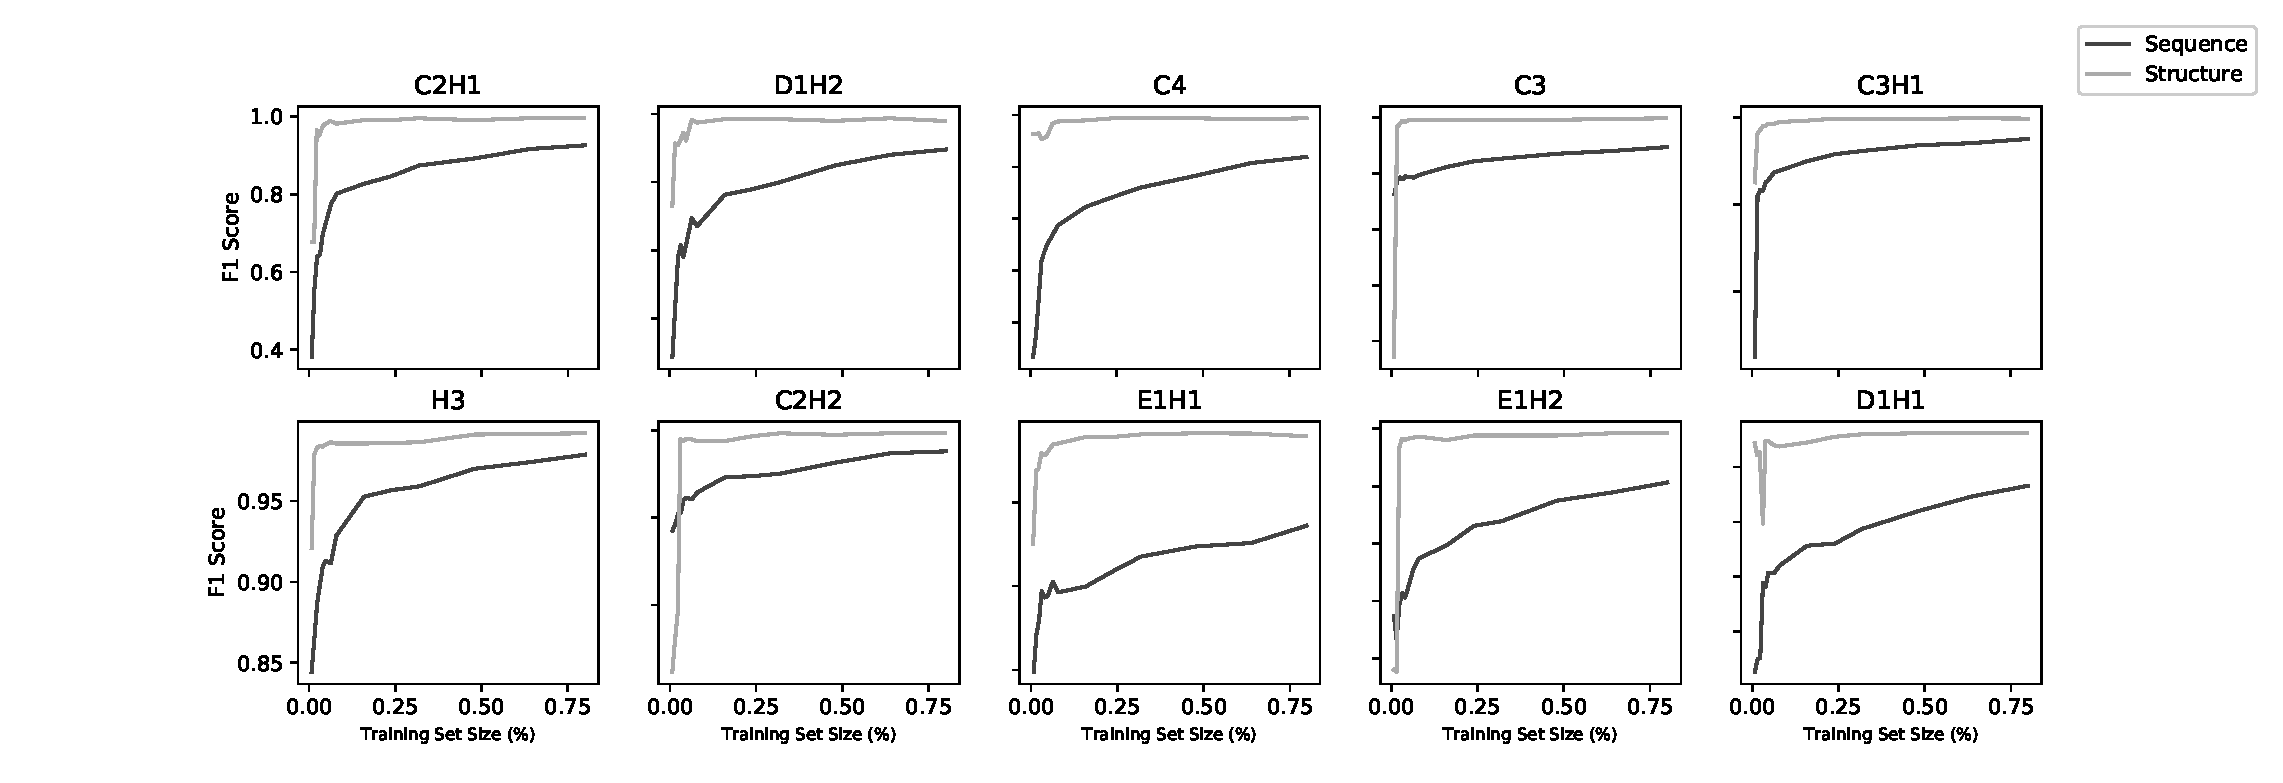
\includegraphics[width=1.0\textwidth]{Figures/learning-curve.eps}
\caption[Learning curves for all 20 models.]{\label{fig:learning-curves} Learning curves for all 20
  models. Each model was trained on increasing subsets of the overall
  training set using five-fold cross-validation. Sequence models
  improved with increasing dataset size, suggesting smaller dataset
  sizes would not be feasible, whereas structure models did not.}
\end{figure}

While the training is affected by dataset size, this does not appear to be a significant limiting factor for most of the models here. Figure~\ref{fig:size-score} shows the model performance (as MCC) for the sequence and structure models. The performance of the sequence models falls off as the dataset falls below a threshold number of data points in the low thousands --- as does the performance of the structural models. The lowest three performing structural models were also the lowest three in dataset size (C3, E1H1, D1H1), but two of these have only two residues so, as discussed above, the performance might not be expected to be very good.

Learning curves (Figure~\ref{fig:learning-curves}) using fractions of the datasets show a correlation with dataset size for the sequence models, but above around 1000 sequences, the structure models do not improve with larger datasets.

The level of abstraction used to describe both sequences and structures made it unlikely that any homology between data in the training and testing sets would artificially improve the performance. The features are largely calculated from residues around the binding residues, rather than the sequence in which they occur. However given the presence of similar sequences in the dataset, I thought it prudent to confirm that these were not artificially increasing the models' performance.

To this end, I wanted to explore what would happen if only unique sequences were used, whereby the available sequences are clustered on some similarity threshold, and one representative from each used. Different sequence identity thresholds were used for clustering with CD-HIT and a training set was created from this new set of sequences for each threshold, and used to create a model. When clustering at 40\% sequence identity (the lowest used), there was slightly lower performance but clustering at this level did result in smaller datasets. As indicated previously, this is a major determinant of these sequence models' performance, so I wanted to determine if this lowered performance was because the dataset size was smaller (which would mean the original models trained on all the data were not compromised) or if a model trained on unique sequences performed less well, which would call into question the high scores of my models as being due to such sequences.

\begin{figure}
\centering
\includegraphics[width=1.0\textwidth]{Figures/clustering.eps}
\caption[MCC as a function of dataset size for 160 different models.]{\label{fig:clustering} MCC as a function of dataset size for
  160 different models.
  For each of the ten zinc-binding families, we trained a
  classifier on 20\%, 30\%, 40\%, 50\%, 60\%, 70\%, 80\%, 90\% and
  100\% of the original, unclustered data, and also a classifier
  trained on data with sequences clustered by 40\%, 50\%, 60\%, 70\%,
  80\%, 90\% and no clustering. Each of these models is shown here,
  with their performance (MCC) and size of the dataset used to train
  them. The two modes of dataset reduction are shown by different
  shades and it can be seen that the curves are not significantly
  different. A
  model's performance is a function of its dataset size, regardless of
  whether any removal of similar sequences is performed.}
\end{figure}

In order to identify whether this lowered performance was because the models performed worse without the possibility of homologous sequences between the training and test sets, or whether it was a result of the smaller training set,
for each zinc-binding family I trained a classifier on 20\%, 30\%, 40\%, 50\%, 60\%, 70\%, 80\%, 90\% and 100\% of the
original, unclustered data, and also a classifier trained on data with sequences clustered by 40\%, 50\%, 60\%, 70\%, 80\%, 90\% and with no clustering. The performance of the models was then plotted against the resulting dataset sizes as shown in Figure~\ref{fig:clustering}.  This demonstrates that it is dataset size that determines model performance, regardless of the similarity of the sequences in the training and testing datasets. For a given dataset, you could predict how well the model trained on it would perform based on dataset size alone --- the similarity of the sequences within that dataset made no difference when dataset size was held constant.

\begin{table}
  \caption{\label{tab:psiblast}Predictive ability of using BLAST alone
    to predict zinc binding in protein sequences using homology
    alone.}
\begin{center}
\begin{tabular}{llllll} \hline
Family & Dataset Size & Recall & Precision & F1    &  MCC  \\ \hline
C2H2   & 3960         & 0.99   & 0.95      & 0.97  &  0.94 \\
C3H1   & 9710         & 0.29   & 0.87      & 0.44  &  0.33 \\
C2H1   & 2154         & 0.24   & 0.88      & 0.37  &  0.3  \\
D1H1   & 818          & 0.05   & 0.8       & 0.09  &  0.11 \\
C3     & 2868         & 0.13   & 0.61      & 0.21  &  0.07 \\ 
E1H1   & 828          & 0.06   & 0.62      & 0.11  &  0.06 \\
D1H2   & 2470         & 0.03   & 0.53      & 0.06  &  0.01 \\
H3     & 5058         & 0.01   & 0.19      & 0.02  & -0.1  \\
E1H2   & 2648         & 0.02   & 0.33      & 0.04  & -0.06 \\ \hline
\end{tabular}
\end{center}
\end{table}

As an additional means of showing how little effect sequence similarity has on ability to predict zinc binding, I compared the sequence models with using BLAST for predicting zinc-binding sites. For each zinc-binding family, a BLAST database was created using 80\% of the available zinc-binding sequences, and BLAST's ability
to identify zinc binding sites from the remaining 20\% was compared against an equivalently sized negative set. Results are shown in Table~\ref{tab:psiblast}. With the exception of C2H2, using BLAST to find zinc binding based on homology performs much worse than the models presented here. Even in the case of C2H2, which seems to have much more similar sequences in its dataset, my model still narrowly outperforms BLAST.

However the models presented here are not intended to be general purpose zinc binding predictors that detect common properties of all zinc binding sites --- they are family-specific predictors based on the principle that common, specific types of zinc binding site have more identifiable, consistent properties than do zinc binding sites in general. As a result, they will not readily detect binding sites of uncommon zinc-binding families. This abstract predictiveness has been deliberately discarded to create highly effective models for specific, common families of zinc binding sites. It is also noteworthy that the binding site itself is a useful unit of prediction using this
methodology --- even for sequences --- rather than individual binding sites. The models are therefore identifying something biologically real (a zinc binding site) rather than something which does not actually exist in isolation (a single zinc binding residue), but which is a useful heuristic in some circumstances.

\begin{table}
  \caption[Percentage of genome predicted to be zinc binding by ZincBindPredict for an assortment of bacterial genomes.]{\label{tab:genome}Percentage of genome predicted to be zinc
    binding by ZincBindPredict for an assortment of bacterial
    genomes. Genomes were acquired from ensembl
    \cite{yates2020ensembl} in the form of translated polypeptide
    sequences, with a sequence labelled as zinc binding if any of the
    ten models finds at least one zinc binding site for that
    sequence/family combination.}
\begin{center}
\begin{tabular}{ll} \hline
Species                          & Percentage of Genome   \\
                                 & Predicted Zinc Binding \\ \hline
{\it Campylobacter jejuni}       & 6.4\%                  \\
{\it Clostridioides difficile}   & 5.8\%                  \\
{\it Enterococcus faecalis}      & 7.5\%                  \\
{\it Listeria monocytogenes}     & 7.9\%                  \\
{\it Mycobacterium tuberculosis} & 11.3\%                 \\
{\it Salmonella enterica}        & 11.1\%                 \\
{\it Shigella flexneri}          & 10.1\%                 \\ 
{\it Streptococcus pneumoniae}   & 7.6\%                  \\ \hline

\end{tabular}
\end{center}
\end{table}

A demonstration of this can be seen by applying the sequence models to bacterial genomes to measure the proportion of typical genomes that the models predict to be zinc binding, as shown for a range of bacterial genomes in Table~\ref{tab:genome}. For most genomes, fewer than 10\% of proteins are flagged as zinc binding, with the average for the genomes examined being 8.46\%. Given that the zinc-binding families for which predictors have been generated represent 67.0\% of binding sites in ZincBindDB, this would imply a `true' predicted proportion of 12.6\% which is a little higher than the widely cited figure of 10\%.

\section{Access to Models}

The models are available through a web app called ZincBindPredict. This is a GraphQL API, like the ZincBindDB database API, which allows users to submit jobs and get the results. A GraphQL request can be sent with either a protein sequence or protein structure, and a job ID will be returned (see Figure~\ref{fig:zbp-mutation}). This can then be polled for results as the protein or sequence is searched using each model in turn, with the identified binding sites returned as a list with the associated probability (see Figure~\ref{fig:zbp-query}). Internally, when a protein is submitted a `job' folder is created, using the current UNIX time in milliseconds as the ID. This job ID is returned to the user, which they can use to query the status of the job, as a script which runs each of the model in turn runs as a background process and saves its results to the job's folder on the server, for inspection by the API.

The ZincBind web interface that was explored in-depth in Chapter 4 also has a page that allows users to submit jobs using a more human-friendly interface, which itself consumes the ZincBindPredict API (see Figure~\ref{fig:prediction-interface}). The user is prompted to provide the representation of a protein - either as a structure file, a sequence file, or a FASTA sequence pasted in. They also have the option of only searching for specific families. Positive results are listed on a results page once the job is complete, and the number of rejected residue combinations is listed.

\begin{figure}
\centering
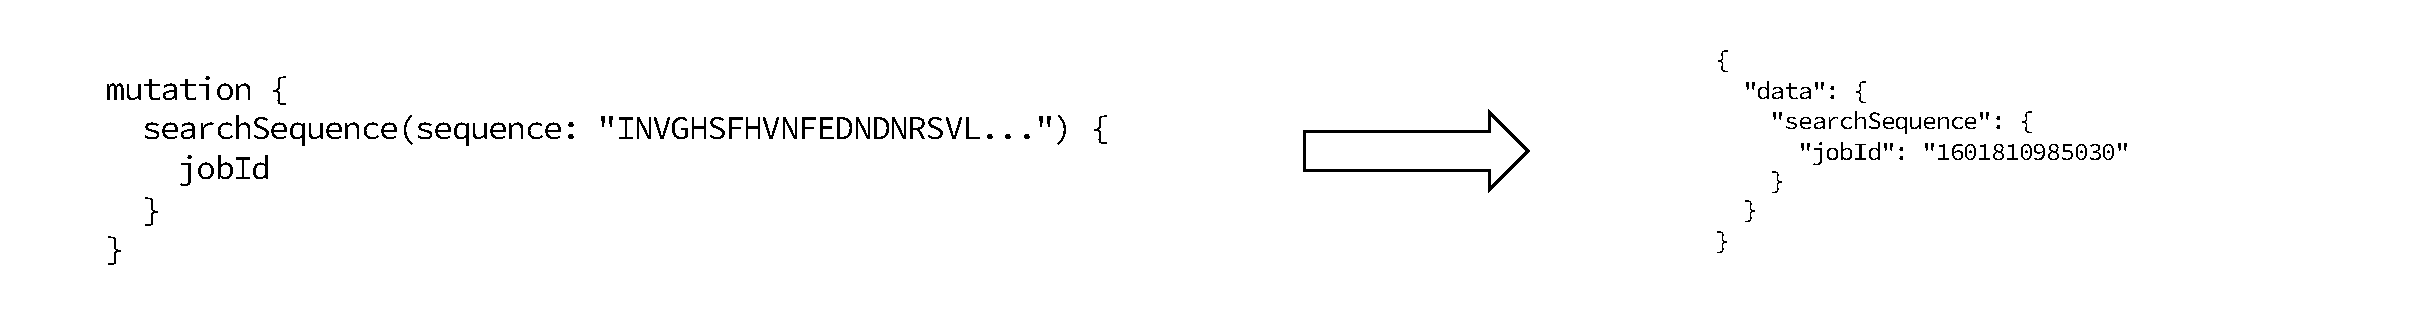
\includegraphics[width=1.0\textwidth]{Figures/zbp-mutation.eps}
\caption[ZincBindPredict mutation request.]{\label{fig:zbp-mutation} A mutation from the ZincBindPredict API. Mutations
begin with the mutation identifier to indicate that the top level \texttt{Mutation} object
is what the \texttt{searchSequence} mutation belongs to --- queries can begin with
\texttt{query} too but this is optional. Here the sequence is being given as an
argument, and the ID of the job is returned.}
\end{figure}

\begin{figure}
\centering
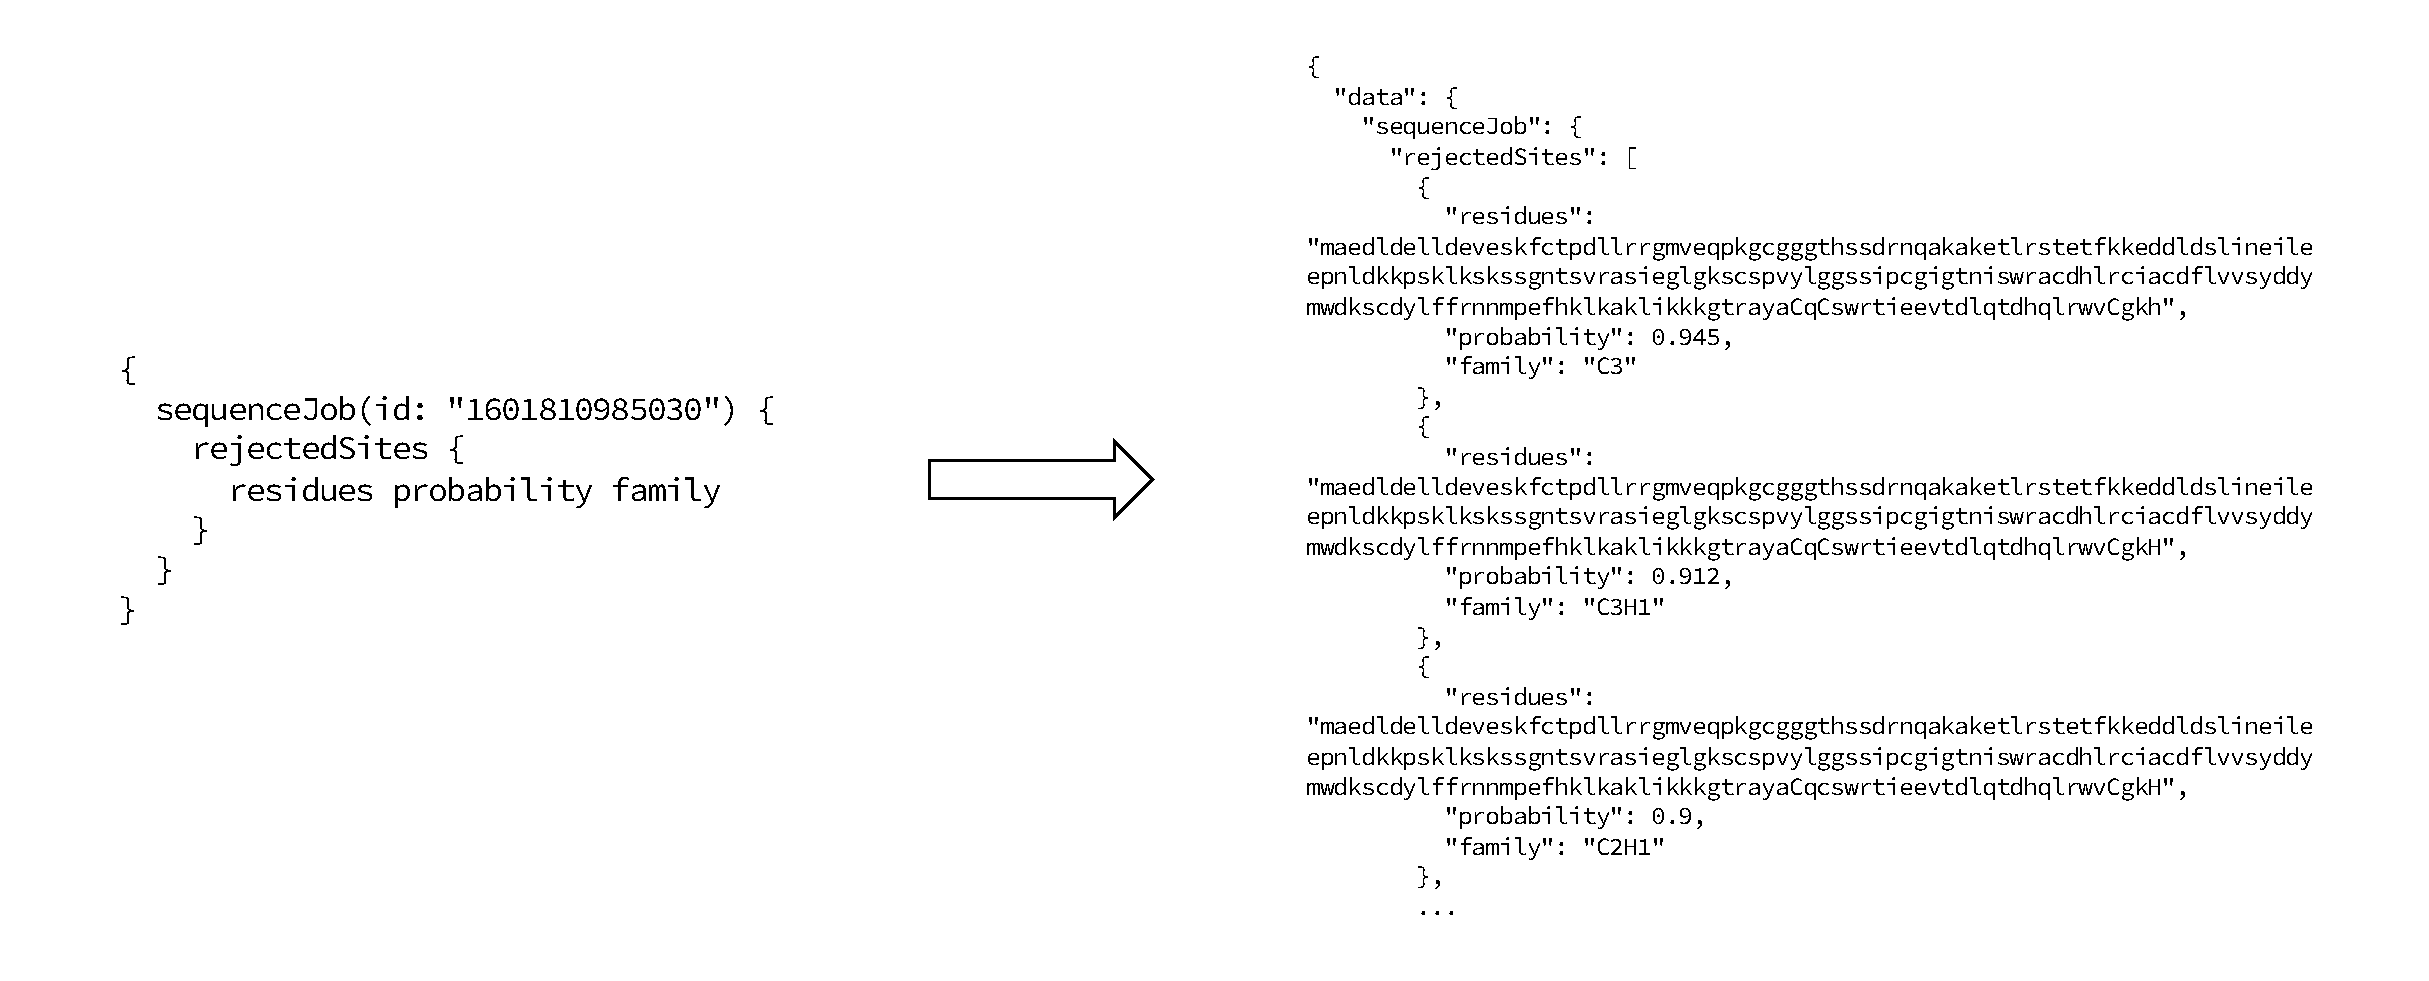
\includegraphics[width=1.0\textwidth]{Figures/zbp-query.eps}
\caption[ZincBindPredict query request.]{\label{fig:zbp-query} A query for the results of a ZincBindPredict job.
The ID of the job is supplied, and this particular query requests the status of
the job, as well the predicted sites. The rejected sites can also be requested,
but since they are quite numerous, typically the flexibility of GraphQL in allowing
you to choose to omit them is useful in conserving network resources.}
\end{figure}

\begin{figure}
\centering
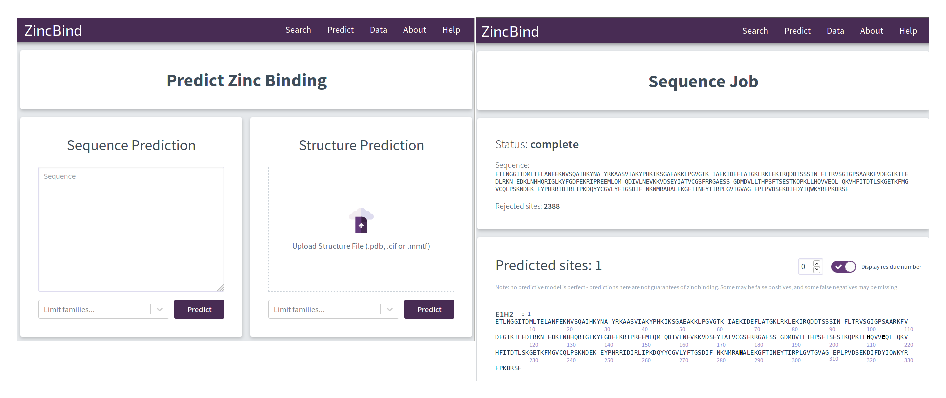
\includegraphics[width=1.0\textwidth]{Figures/prediction-interface.eps}
\caption[The prediction page on the ZincBind web interface.]{\label{fig:prediction-interface} The prediction page on the ZincBind web interface, and an example of a predicted zinc binding site in a protein sequence.}
\end{figure}

\section{Conclusion}

The models created here are highly effective, albeit at a very particular task. They are not predictors of zinc binding in general, and they will not generally detect zinc binding sites of obscure families and residue combinations. They were never intended to. A deliberate trade-off between model effectiveness and model generalisability has been made in order to demonstrate the principal that properties of binding sites within families \emph{are} more tightly distributed and hence create more accurate models. These models also detect something biologically real --- full binding sites --- rather than individual zinc binding residues which, as discussed, are an artificial concept.

However, this downside is not necessarily permanent. The models are limited to these ten models because these are the families for which there is sufficient (only just, in the case of some of the sequence models) data to train a classifier. However, the data in ZincBind is constantly growing thanks to the automated database update scripts in place. Over the time, the eleventh-placed model will acquire enough data to warrant a model, and then the twelfth, and so on. The dataset-size threshold for training is not relative to the total size of the database, it is an absolute amount, and so over time more and more families will be able to have models trained for them, and the models will become more comprehensive of zinc binding generally. The benefits of this trade-off are permanent --- the deficiencies are temporary.







%%%%% MACRO DEFINITION %%%%

\providecommand{\pvivax}{P.~vivax}
\providecommand{\pfalciparum}{P.~falciparum}
\providecommand{\cterm}{C-terminus}
\providecommand{\nterm}{N-terminus}

\providecommand{\e}[1]{\ensuremath{\times 10^{#1}}}
\newcolumntype{P}[1]{>{\centering\arraybackslash}p{#1}}
\newcolumntype{M}[1]{>{\centering\arraybackslash}m{#1}}

\providecommand{\refimage}[1]{\figurename~\ref{fig:#1}}

%TC:macro \note [ignore]



%%%%%%%%%%%%%%%%%%%%%%%%%%%%%%%%%%%%%%%%%%%%%%%%%%%%%%%%%%%%%%%%%%%%%%%%%%%%%%%%%%%%%%%%%%%%%%%%%%%%%%%%%%%%%%%%%%%%%
%%%%%%%%%%%%%%%%%%%%%%%%%%%%%%%%%%%%%%%%%%%%%%%%%%%%%%%%%%%%%%%%%%%%%%%%%%%%%%%%%%%%%%%%%%%%%%%%%%%%%%%%%%%%%%%%%%%%%
%													BEGIN
%%%%%%%%%%%%%%%%%%%%%%%%%%%%%%%%%%%%%%%%%%%%%%%%%%%%%%%%%%%%%%%%%%%%%%%%%%%%%%%%%%%%%%%%%%%%%%%%%%%%%%%%%%%%%%%%%%%%%
%%%%%%%%%%%%%%%%%%%%%%%%%%%%%%%%%%%%%%%%%%%%%%%%%%%%%%%%%%%%%%%%%%%%%%%%%%%%%%%%%%%%%%%%%%%%%%%%%%%%%%%%%%%%%%%%%%%%%

\chapter{Conclusion} % Write in your own chapter title
\label{Chapter6}
\lhead{Chapter 6. \emph{Conclusion}} % Write in your own chapter title to set the page header

This PhD has been an investigation into the properties of high affinity zinc binding sites in proteins, and the extent to which these properties can be used to create predictive models of zinc binding from protein structures or protein sequences.

Investigations of this kind into the nature of zinc binding are of importance at a basic research level, and in a direct medical sense. Understanding the geometric and biochemical properties of zinc binding sites offers insights into how they function - whether that function is catalytic or structure stabilising. Correspondingly, being able to determine whether a protein binds zinc can offer insights into what the function of that protein is - particularly if the location can be determined too. This is particularly effective in models which can predict from sequence, because entire genomes can be screened in minutes or hours to identify what zinc binding proteins might be present. Medically, the association of pathological zinc binding --- particularly in the eye --- is a demonstration of how vital a detailed understanding of the mechanisms of zinc binding is to understanding these diseases, and in how predicting the locations of binding sites can be used to aid pharmaceutical interventions.

This project, while an interesting intellectual exercise in and of itself, has been carried out with these crucial benefits to our understanding of the role of zinc in protein functions in health and disease at all times.

Understanding of the properties of zinc binding has been expanded by creating a more comprehensive database of all known zinc binding sites than previous research has created. The key properties and characteristics gleaned from Chapter 4 will not be repeated here, but they largely expanded in more detail on some properties that were already commented upon by previous works.

Probably a much more fundamental contribution to the future of this field, is the existence of ZincBindDB not as a closed dataset that exists on a PhD Researcher's laptop and which can possibly, after an exchange of emails, be made available to other individuals ---  but rather a web accessible, continually updated resource that has both a web API and web interface. The vast majority of previous research of this has kind has resulted in datasets of the former kind, which are not easily shared among researchers and which are in any case static once created. The data generated here is very easily accessed by any researcher in the world without the need for my involvement at all, and will continue to be updated with the very latest zinc binding structures indefinitely.

Similarly, those previous works which did result in a web interface have almost all ceased to exist. Even relatively recent papers from the mid-2010s contain URLs which, when accessed in 2021, point to nothing. Nobody can guarantee that they will maintain a service forever --- particularly in the academic sciences where such services are funded by single standalone grants rather than revenue generated by those services. In this case however, all components of ZincBind are open source, cloneable, and reproducible. Even if neither I nor my lab continued to maintain ZincBind (it is currently very much the intention to do so), another researcher could recreate both the services and the data they contained very easily via the GitHub repositories and Docker images, rather than having to recreate from scratch using the Methods section of a paper.

Over the long term, the particular insights into the properties of zinc binding that this PhD has uncovered will be expanded upon and may in some instances be superseded, but the long term presence and availability of this dataset via ZincBind may yet be the most important lasting contribution to the field of zinc binding.

The machine learning component of the PhD has, like the database creation component, built upon previous, similar studies. Here however the difference in methodology has been more stark. From the outset I deliberately departed from two ubiquitous assumptions that these previous works made --- that zinc binding was best detected at the individual residue level, and that the properties of zinc binding sites did not vary much between sub-categories of binding site. The reasons for doubting the validity of these assumptions were explored in Chapter 5 and will not be repeated here. The conclusion however is worth repeating --- by making this tradeoff of only searching for a subset of zinc binding sites, you can achieve superior results in the prediction of zinc binding, and that this tradeoff will become less severe as time passes and the size of the underlying database grows.

Finally, this PhD has resulted in the creation of the Python library atomium for processing PDB structures. This library is already seeing use in the wider field and will continue to be updated with features.

\section{Next Steps}

It is worth examining, in closing, what the logical next steps would be were this project to continue. One very useful extension has already been remarked upon in chapter 5 and indeed will likely happen with very little input from the author or anyone else --- the expansion of the predictive models beyond the existing ten. As chapter 5 explained in detail, there is currently enough data to justify these ten, but insufficient data for any more. As ZincBindDB is automatically updated every week from the Protein Data Bank, over time other families will cross the threshold of data size for these to have predictive models too, and the coverage of the models will gradually increase. This will simply require retraining the models, and adding families to the .dat file used by the build scripts. This will improve the usefulness of the tools over time.

Another possible expansion of the work done here that would have a rather high resultant benefit to effort required ratio, would be to expand beyond just zinc, to other metals. Because the primary objective of the original database creation was to identify properties of zinc binding sites, no previously identified properties were used in creating the database --- the build scripts simply looks for PDB ligands with the name ZN and identifies binding sites for them based on general principles of atomic interactions (sensible atom distance thresholds, minimum angles for atom clashing, etc.). Because nothing about this is specific to zinc, everything done here could just as easily be done for, as an example, copper, or iron. The only restriction used in looking for liganding atoms was the rejection of carbon as a possible liganding atom, but this will be true of all metals. Once this database of all transition metal binding sites were created, likewise creating predictive models for them would also require little to no changes to the already developed codebases. This was not done as part of this PhD to keep it tightly focused on the original research question and not allow for `mission creep' --- but it would greatly increase the usefulness of the already developed code with very little extra work.

An additional possible future avenue for research would be to try and create predictive models of a particular kind of zinc binding site - partial binding sites. These are those binding sites formed of multiple protein chains, in which often the zinc contributes to the oligomerisation of multiple subunits. Predicting these would be particularly useful in the aforementioned pathological aggregation of proteins in the presence of zinc, which is caused by cryptic half-binding sites in the proteins in question. Creating models that detect these is a much more difficult proposition, because it is very difficult to create a correctly labelled dataset. Positive samples are easily enough identified from ZincBindDB by filtering binding sites to include those from multiple chains --- although they are less numerous than the singe chain sites used here. Identifying negative samples is much more difficult though. The very nature of these sites means that unless a protein is crystallised in the presence of zinc and in the presence of a protein chain that could make up the other half of a binding site, it will go undetected. There is no easy way to reliably confirm that a pair of residues in a structure could not form a half binding site, simply because it does not in a particular structure, which means the methodology used here would not be suitable. That is not to say there is not path towards doing this, but unlike the previous two proposed future extensions, this could not be done by simply making superficial changes to existing code.

Other suggested features have been made by various interested parties over the course of the PhD --- automatic classification of binding sites as structural or catalytic (sites are not labelled as such in PDB files, but they seem to have very different properties so a dataset could be constructed with some effort), and prediction of binding site affinity (again this might be limited by the amount of available experimental data) to name two that would be of particular use. Ultimately the best way to decide how future effort would best be spent is to be guided by the actual needs of people using the existing tools. All of the software created as part of this project is open source, and available on GitHub with its associated issue trackers and feature request managers. These offer a much more concrete guide to what would be most useful to the community, and is broadly the approach that will be taken in future.


%\include{Chapter_7}


%% ----------------------------------------------------------------
% Now begin the Appendices, including them as separate files

\addtocontents{toc}{\vspace{2em}} % Add a gap in the Contents, for aesthetics

\appendix % Cue to tell LaTeX that the following 'chapters' are Appendices

%%%% MACRO DEFINITION %%%%
% if any ...


%%%%%%%%%%%%%%%%%%%%%%%%%%%%%%%%%%%%%%%%%%%%%%%%%%%%%%%%%%%%%%%%%%%%%%%%%%%%%%%%%%%%%%%%%%%%%%%%%%%%%%%%%%%%%%%%%%%%%
%													BEGIN
%%%%%%%%%%%%%%%%%%%%%%%%%%%%%%%%%%%%%%%%%%%%%%%%%%%%%%%%%%%%%%%%%%%%%%%%%%%%%%%%%%%%%%%%%%%%%%%%%%%%%%%%%%%%%%%%%%%%%


\chapter{Publications and Talks} % Write in your own chapter title
\lhead{Appendix. \emph{A}} % Write in your own chapter title to set the page header

%TC:macro \note [ignore]

% write your code here

\section{Published Papers}

The following papers have been published from this PhD:

\subsection{ZincBind—the database of zinc binding sites}

\emph{5 February 2019}

Abstract: Zinc is one of the most important biologically active metals. Ten per cent of the human genome is thought to encode a zinc binding protein and its uses encompass catalysis, structural stability, gene expression and immunity. At present, there is no specific resource devoted to identifying and presenting all currently known zinc binding sites. Here we present ZincBind, a database of zinc binding sites and its web front-end. Using the structural data in the Protein Data Bank, ZincBind identifies every instance of zinc binding to a protein, identifies its binding site and clusters sites based on 90% sequence identity. There are currently 24 992 binding sites, clustered into 7489 unique sites. The data are available over the web where they can be browsed and downloaded, and via a REST API. ZincBind is regularly updated and will continue to be updated with new data and features.


\subsection{atomium—a Python structure parser}

\emph{11 February 2020}

Abstract: Structural biology relies on specific file formats to convey information about macromolecular structures. Traditionally this has been the PDB format, but increasingly newer formats, such as PDBML, mmCIF and MMTF are being used. Here we present atomium, a modern, lightweight, Python library for parsing, manipulating and saving PDB, mmCIF and MMTF file formats. In addition, we provide a web service, pdb2json, which uses atomium to give a consistent JSON representation to the entire Protein Data Bank. atomium is implemented in Python and its performance is equivalent to the existing library BioPython. However, it has significant advantages in features and API design. atomium is available from atomium.bioinf.org.uk and pdb2json can be accessed at pdb2json.bioinf.org.uk.


\subsection{Zincbindpredict—Prediction of Zinc Binding Sites in Proteins}

\emph{12 February 2021}

Abstract: Zinc binding proteins make up a significant proportion of the proteomes of most organisms and, within those proteins, zinc performs rôles in catalysis and structure stabilisation. Identifying the ability to bind zinc in a novel protein can offer insights into its functions and the mechanism by which it carries out those functions. Computational means of doing so are faster than spectroscopic means, allowing for searching at much greater speeds and scales, and thereby guiding complimentary experimental approaches. Typically, computational models of zinc binding predict zinc binding for individual residues rather than as a single binding site, and typically do not distinguish between different classes of binding site—missing crucial properties indicative of zinc binding. Previously, we created ZincBindDB, a continuously updated database of known zinc binding sites, categorised by family (the set of liganding residues). Here, we use this dataset to create ZincBindPredict, a set of machine learning methods to predict the most common zinc binding site families for both structure and sequence. The models all achieve an MCC $\ge$ 0.88, recall $\ge$0.93 and precision $\ge$0.91 for the structural models (mean MCC = 0.97), while the sequence models have MCC $\ge$ 0.64, recall $\ge$0.80 and precision $\ge$0.83 (mean MCC = 0.87), with the models for binding sites containing four liganding residues performing much better than this. The predictors outperform competing zinc binding site predictors and are available online via a web interface and a GraphQL API.


\section{Talks and Presentations}

This PhD has been presented on the following occasions:

\begin{itemize}
  \item 12 June 2018 --- ISMB Graduate Symposium.
  \item 22 February 2019 --- ISMB Friday Wrap.
  \item 24 January 2020 --- GRC Metals in Biology Conference, Ventura, California.
  \item 6 March 2020 --- ISMB Friday Wrap.
  \item 11 October 2020 --- Exscientia (remote presentation).
  \item 15 October 2020 --- Vernalis (remote presentation).
  \item 15 January 2021 --- ISMB Friday Wrap (remote presentation).
\end{itemize}

%%%%%%%%%%%% END %%%%%%%%%%%%
	% Appendix Title
\include{Appendix_B}	% Appendix Title


\addtocontents{toc}{\vspace{2em}}  % Add a gap in the Contents, for aesthetics
\backmatter

%% ----------------------------------------------------------------
\label{Bibliography}
\lhead{\emph{Bibliography}}  % Change the left side page header to "Bibliography"
%\bibliographystyle{unsrtnat}  % Use the "unsrtnat" BibTeX style for formatting the Bibliography
\bibliographystyle{ieeetr}  % Use the "unsrtnat" BibTeX style for formatting the Bibliography
\bibliography{Bibliography}  % The references (bibliography) information are stored in the file named "Bibliography.bib"

\end{document}  % The End
%% ----------------------------------------------------------------
